\documentclass[tikz,border=10pt]{standalone}
\begin{document}
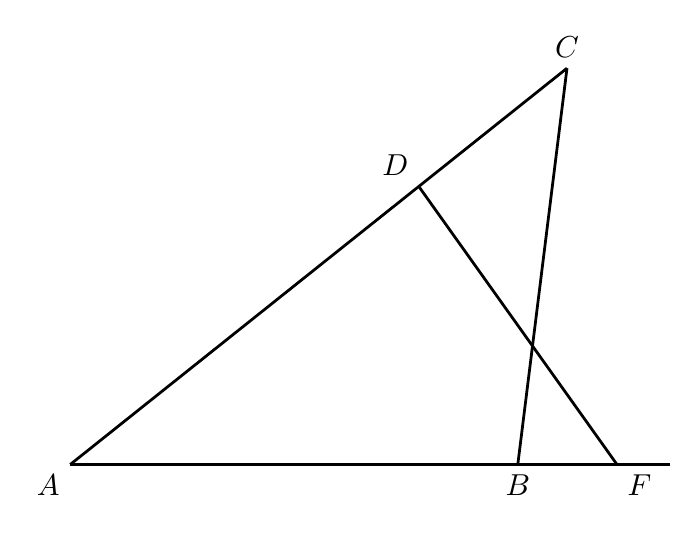
\begin{tikzpicture}[line join=round, line width=1.0pt]
% Scale s=0.008909 cm/px, centre (526,386.5) px; y flipped
\coordinate (A) at (-3.600,-2.392);
\coordinate (B) at (2.084,-2.392);
\coordinate (F) at (3.344,-2.392);
\coordinate (E) at (4.018,-2.392);   % baseline overhang end (977 px, kept per GES)
\coordinate (C) at (2.709,2.641);
\coordinate (D) at (0.827,1.139);

% Line C-D-A (D lies on it)
\draw (C) -- (A);
% Side C-B
\draw (C) -- (B);
% Baseline A-F (continues past F)
\draw (A) -- (E);
% Segment D-F
\draw (D) -- (F);

% Labels
\node[below left]  at (A) {\fontsize{11}{13.2}\selectfont $A$};
\node[below]       at (B) {\fontsize{11}{13.2}\selectfont $B$};
\node[below right] at (F) {\fontsize{11}{13.2}\selectfont $F$};
\node[above]       at (C) {\fontsize{11}{13.2}\selectfont $C$};
\node[above left]  at (D) {\fontsize{11}{13.2}\selectfont $D$};
\end{tikzpicture}
\end{document}